\chapter{Background}

\section{Cumulus Clouds}
In the Introduction section of the paper, the author introduced their method and their rendering target briefly. I'm writing this section to supplement his introduction.

\subsection{What is cumulus clouds?}

\begin{figure}[htp]
\begin{center}

\includegraphics[scale=0.1]{images/single-fluffy-cumulus-cloud-sunny-day-2012-07-26.jpg}
\caption{Single cumulus cloud}
\label{f1}
\end{center}
\end{figure}

Cumulus clouds is a type of clouds which is fairly close to the ground with an observable volume and visible and clear edges. Comulus clouds are often been noticed as "puffy" or "cotton" in the appearance, and they also generally have flat bases. As a low-stage kind of clouds, the general altitude of the cumulus clouds are less than meters, unless they are in the more vertical cumulus congestus form. As for the appearance, cumulus clouds usually appear by themselves, in certain forms, such as lines and clusters.

\subsection{Why does the paper concentrate on rendering cumulus clouds?}
Among the numerous kinds of clouds in the nature environment, cumulus clouds have the most pronounced volumetric feature, making the volumetric rendering more practical. In the final step of the proposed method from the paper, a volume-aware blending is performed. If we use other kind of clouds, such as stratus clouds or cirrus clouds, the volumetric feature can be hardly found, which is not able to be rendered as physically based clouds. This is because we will need a volume to calculate the light occlusion later on.

\section{Existing cloud rendering techniques}
The author of the paper talked about the related work that has been down and from his research we know that off-line rendering can be quite accurate about simulating the cloud, but it could take minutes to hours to draw a single frame. We'll be looking into the existing real time rendering methods in detail in this section.

\subsection{Particle Systems (Billboards)}
\begin{figure}[htp]
\begin{center}
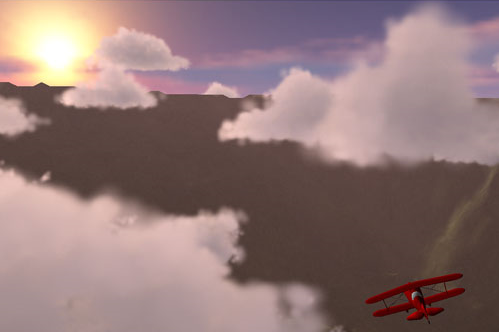
\includegraphics[scale=0.6]{images/billboards.png}
\caption{Billboards Clouds}
\label{f2}
\end{center}
\end{figure}

Particles in video game industry are referenced as small units with independent rotations, and they are usually rendered by using a textured quad which represents the projection onto the view plane. They are rendered in back-to-front order, and also the blending for semi-transparent volumes are applied.\\
By rendering clouds with billboards as particle system, we treat the clouds as 3D objects, and they face the camera all the time. We also generate shafts of light by making concentric semi-transparent containers. Here is a typical scenario for a flight game: the player controls an aircraft shuttling in and out of clouds. When the aircraft moves into a cloud, the imposter of that cloud will be split into 2 pieces, one piece in the front of the aircraft, and the other piece behind the aircraft.\\
This method has certain advantages, such as fast, efficient, and the programmer can easily manipulate the shapes and the locations of the billboards. However, as the clouds are represented in a quads facing the camera all the time, the scene will get unrealistic sometimes, for example, when an aircraft flies above the clouds, we will still see the clouds facing the camera as if the we are on the ground. Also the lighting on the billboard is usually precomputed and the clouds are static, which means that the clouds will not be able to adjust its appearance according to the environment's changes.

\subsection{Ray Casting-Based Rendering (Ray Marching)}
\begin{figure}[htp]
\begin{center}

\includegraphics[scale=0.5]{images/raymarching.png}
\caption{Ray Marching Clouds}
\label{f3}
\end{center}
\end{figure}

By rendering clouds in the ray marching method, the typical way is to cast multiple rays into the scene and accumulate the densities of the volume within certain interval distances. We then represent the cloud density with 3D noise images. In order to calculate the illumination values, we usually apply a volume lighting model in real time or we can retrieve the illumination data from a pre-computed lighting structure, such as a look-up table.\\
This method can result in a fairly realistic output. However, it's not easy for a programmer to control the shape and location of the clouds. Also, in order to do aliasing, the ray marching steps will be tedious. As for the rendering result, the lightings is usually limited to single scattering, which is more or less not so realistic.

\subsection{Rasterization-based Rendering (Volume Slicing)}
\begin{figure}[htp]
\begin{center}
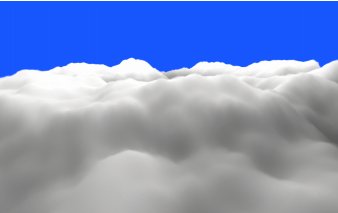
\includegraphics[scale=1.0]{images/volumerendering.png}
\caption{Volume Rendering Clouds}
\label{f4}
\end{center}
\end{figure}

In terms of rasterization-based rendering, volume slicing is the most realistic method for rendering clouds.\\
Volume slicing is quite straightforward, and it is used for rendering regular grids. The slices of the volume are usually aligned to XYZ axes and they are rendered in front-to-back or back-to-front order. Finally, we apply the view transformations and blending to the rendering pipeline. As we can see, volume slicing is not strictly based on rasterization methods, most algorithms of this field rely on the highly optimized texturing capabilities of the GPU.\\
By using this method, we can have a convincing light result, since it enables the multiple forward light scattering using slices. However, like ray marching method, it's difficult for a programmer to control the shape and location of the clouds. Also, in order to get a more realistic result, the volume will be sliced into tons of planes, which takes a lot of memory and execution time.

\section{Mathematical Background}
The author discussed the concepts of calculating the light transport in a certain medium and the mathematical solution to the concepts. As we know, the light is able to transport in a number of materials, such as air, fluid, and solid medium. Different materials of the medium will result in different amount of scattering and absorption. In clouds simulating, the medium will be small particles.